\section[Rastreabilidade de Requisitos]{Rastreabilidade de Requisitos}
% 
% A rastreabilidade pode ser dividida em pré-rastreabilidade e pós-rastreabilidade. 
% A pré-rastreabilidade consiste no rastreamento de informações anteriores a especificação
% de requisitos. Como por exemplo, a fonte dos requisitos que podem ser: \textit{stakeholders},
% documentos e regras de negócio. Já a pós-rastreabilidade está relacionada com os requisitos depois 
% de serem especificados e está mais focada na solução. \cite{persson}
% 
% A rastreabilidade também pode ser horizontal ou vertical. A horizontal está relacionada com
% as informações de uma mesma fase do processo de desenvolvimento e a vertical
% com informações entre várias fases do processo. \cite{persson}
% 
% De acordo com \citeonline{paetsch}, a rastreabilidade auxilia na gerência de mudanças, 
% pois estabelece um relacionamento entre os requisitos, o projeto e a implementação do sistema. \citeonline{nuseibeh}
% afirmam que a rastreabilidade é o coração do gerenciamento de requisitos.
% 
% No SAFe os requisitos possuem quatro graus diferentes de abstração dos requisitos: tema de investimento, épicos, \textit{features} e histórias.
% A partir disso, a rastreabilidade definida para esse trabalho pode ser vista na Figura \ref{fig:rastreabilidade}.
% Será realizada uma rastreabilidade, através da ferramenta de gerenciamento de requisitos, vertical e horizontal. Assim acompanhando
% a origem das histórias, ou seja, de qual \textit{feature} e épico é derivada e também monitorar as dependências entre as histórias,\textit{features} e épicos.
% 
% Também será realizada a pré-rastreabilidade para identificar a fonte dos requisitos. A rastreabilidade definida será feita através da ferramenta de gerenciamento de requisitos.
% 
% \graphicspath{{figuras/}}
% 
% \begin{figure}[!htb]
%  \centering
%  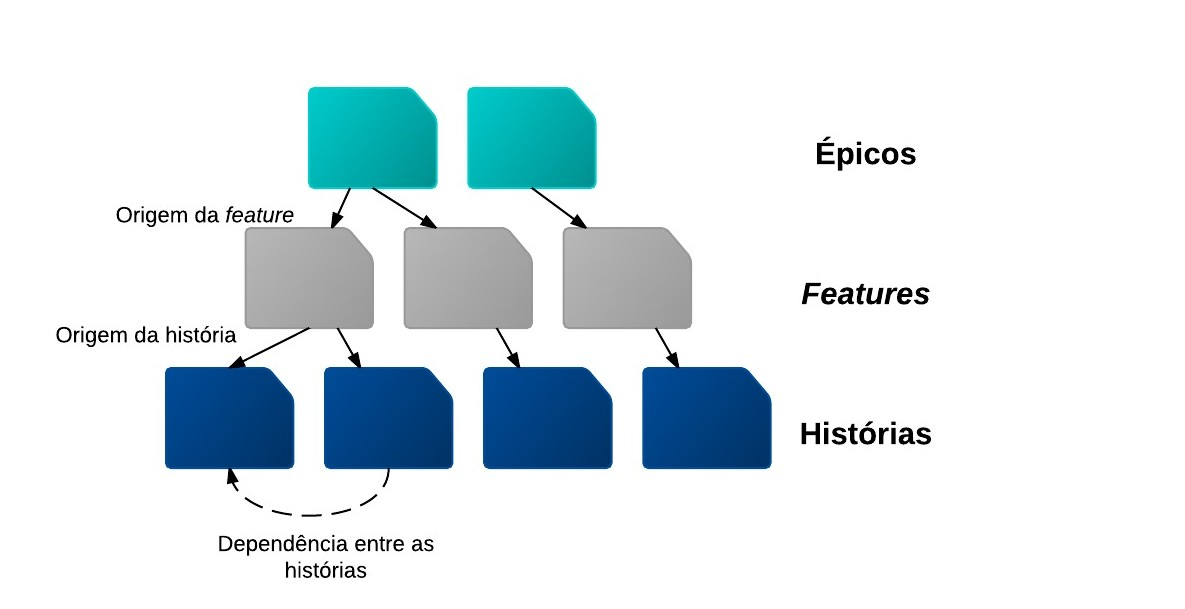
\includegraphics[width = 18cm, height = 15cm]{rastreabilidade}
%  \caption{Estratégia de rastreabilidade baseada no SAFe \cite{safe}}
%  \label{fig:rastreabilidade}
% 
% \end{figure}